%% LyX 2.3.4.2 created this file.  For more info, see http://www.lyx.org/.
%% Do not edit unless you really know what you are doing.
\documentclass[11pt,oneside,american,czech]{book}
\usepackage[T1]{fontenc}
\usepackage[utf8]{inputenc}
\usepackage[a4paper]{geometry}
\geometry{verbose,tmargin=4cm,bmargin=3cm,lmargin=3cm,rmargin=2cm,headheight=0.8cm,headsep=1cm,footskip=0.5cm}
\pagestyle{headings}
\setcounter{secnumdepth}{3}
\usepackage{url}
\usepackage{amsmath}
\usepackage{amsthm}
\usepackage{amssymb}
\usepackage{graphicx}
\usepackage{setspace}

\usepackage{pdfpages}
\usepackage[backend=bibtex]{biblatex}
\addbibresource{ref.bib}

\makeatletter
%%%%%%%%%%%%%%%%%%%%%%%%%%%%%% Textclass specific LaTeX commands.
\newenvironment{lyxlist}[1]
	{\begin{list}{}
		{\settowidth{\labelwidth}{#1}
		 \setlength{\leftmargin}{\labelwidth}
		 \addtolength{\leftmargin}{\labelsep}
		 \renewcommand{\makelabel}[1]{##1\hfil}}}
	{\end{list}}

%%%%%%%%%%%%%%%%%%%%%%%%%%%%%% User specified LaTeX commands.
%% Font setup: please leave the LyX font settings all set to 'default'
%% if you want to use any of these packages:

%% Use Times New Roman font for text and Belleek font for math
%% Please make sure that the 'esint' package is turned off in the
%% 'Math options' page.
\usepackage[varg]{txfonts}

%% Use Utopia text with Fourier-GUTenberg math
%\usepackage{fourier}

%% Bitstream Charter text with Math Design math
%\usepackage[charter]{mathdesign}

%%---------------------------------------------------------------------

%% Make the multiline figure/table captions indent so that the second
%% line "hangs" right below the first one.
%\usepackage[format=hang]{caption}

%% Indent even the first paragraph in each section
\usepackage{indentfirst}

%%---------------------------------------------------------------------

%% Disable page numbers in the TOC. LOF, LOT (TOC automatically
%% adds \thispagestyle{chapter} if not overriden
%\addtocontents{toc}{\protect\thispagestyle{empty}}
%\addtocontents{lof}{\protect\thispagestyle{empty}}
%\addtocontents{lot}{\protect\thispagestyle{empty}}

%% Shifts the top line of the TOC (not the title) 1cm upwards 
%% so that the whole TOC fits on 1 page. Additional page size
%% adjustment is performed at the point where the TOC
%% is inserted.
%\addtocontents{toc}{\protect\vspace{-1cm}}

%%---------------------------------------------------------------------

% completely avoid orphans (first lines of a new paragraph on the bottom of a page)
\clubpenalty=9500

% completely avoid widows (last lines of paragraph on a new page)
\widowpenalty=9500

% disable hyphenation of acronyms
\hyphenation{CDFA HARDI HiPPIES IKEM InterTrack MEGIDDO MIMD MPFA DICOM ASCLEPIOS MedInria}

%%---------------------------------------------------------------------

%% Print out all vectors in bold type instead of printing an arrow above them
\renewcommand{\vec}[1]{\boldsymbol{#1}}

% Replace standard \cite by the parenthetical variant \citep
%\renewcommand{\cite}{\citep}

\makeatother

\usepackage{babel}
\begin{document}
%\def\documentdate{7. \v{c}ervence 2021}

\def\documentdate{\today}

\pagestyle{empty}
{\centering

\noindent %
\begin{minipage}[c]{3cm}%
\noindent \begin{center}

\includegraphics[width=3cm,height=3cm,keepaspectratio]{Images/TITLE/cvut}
\par\end{center}%
\end{minipage}%
\begin{minipage}[c]{0.6\linewidth}%
\begin{center}
\textsc{\large{}České vysoké učení technické v Praze}{\large{}}\\
{\large{}Fakulta jaderná a fyzikálně inženýrská}
\par\end{center}%
\end{minipage}%
\begin{minipage}[c]{3cm}%
\noindent \begin{center}

\includegraphics[width=3cm,height=3cm,keepaspectratio]{Images/TITLE/fjfi}
\par\end{center}%
\end{minipage}

\vspace{3cm}

\textbf{\huge{}Automatická registrace snímků video}{\huge\par}

\vspace{1cm}

\selectlanguage{american}%
\textbf{\huge{}Automatic registration of video
frames}{\huge\par}

\selectlanguage{czech}%
\vspace{2cm}

{\large{}Bakalářská práce}{\large\par}

}

\vfill{}

\begin{lyxlist}{MMMMMMMMM}
\begin{singlespace}
\item [{Autor:}] \textbf{Daniela Lichnovská}
\item [{Vedoucí~práce:}] \textbf{doc. Ing. Filip Šroubek, Ph.D. DSc.}
\item [{Konzultant:}] \textbf{Ing. Lukáš Tryner}
\item [{Akademický~rok:}] 2020/2021
\end{singlespace}
\end{lyxlist}
%\newpage{}

~

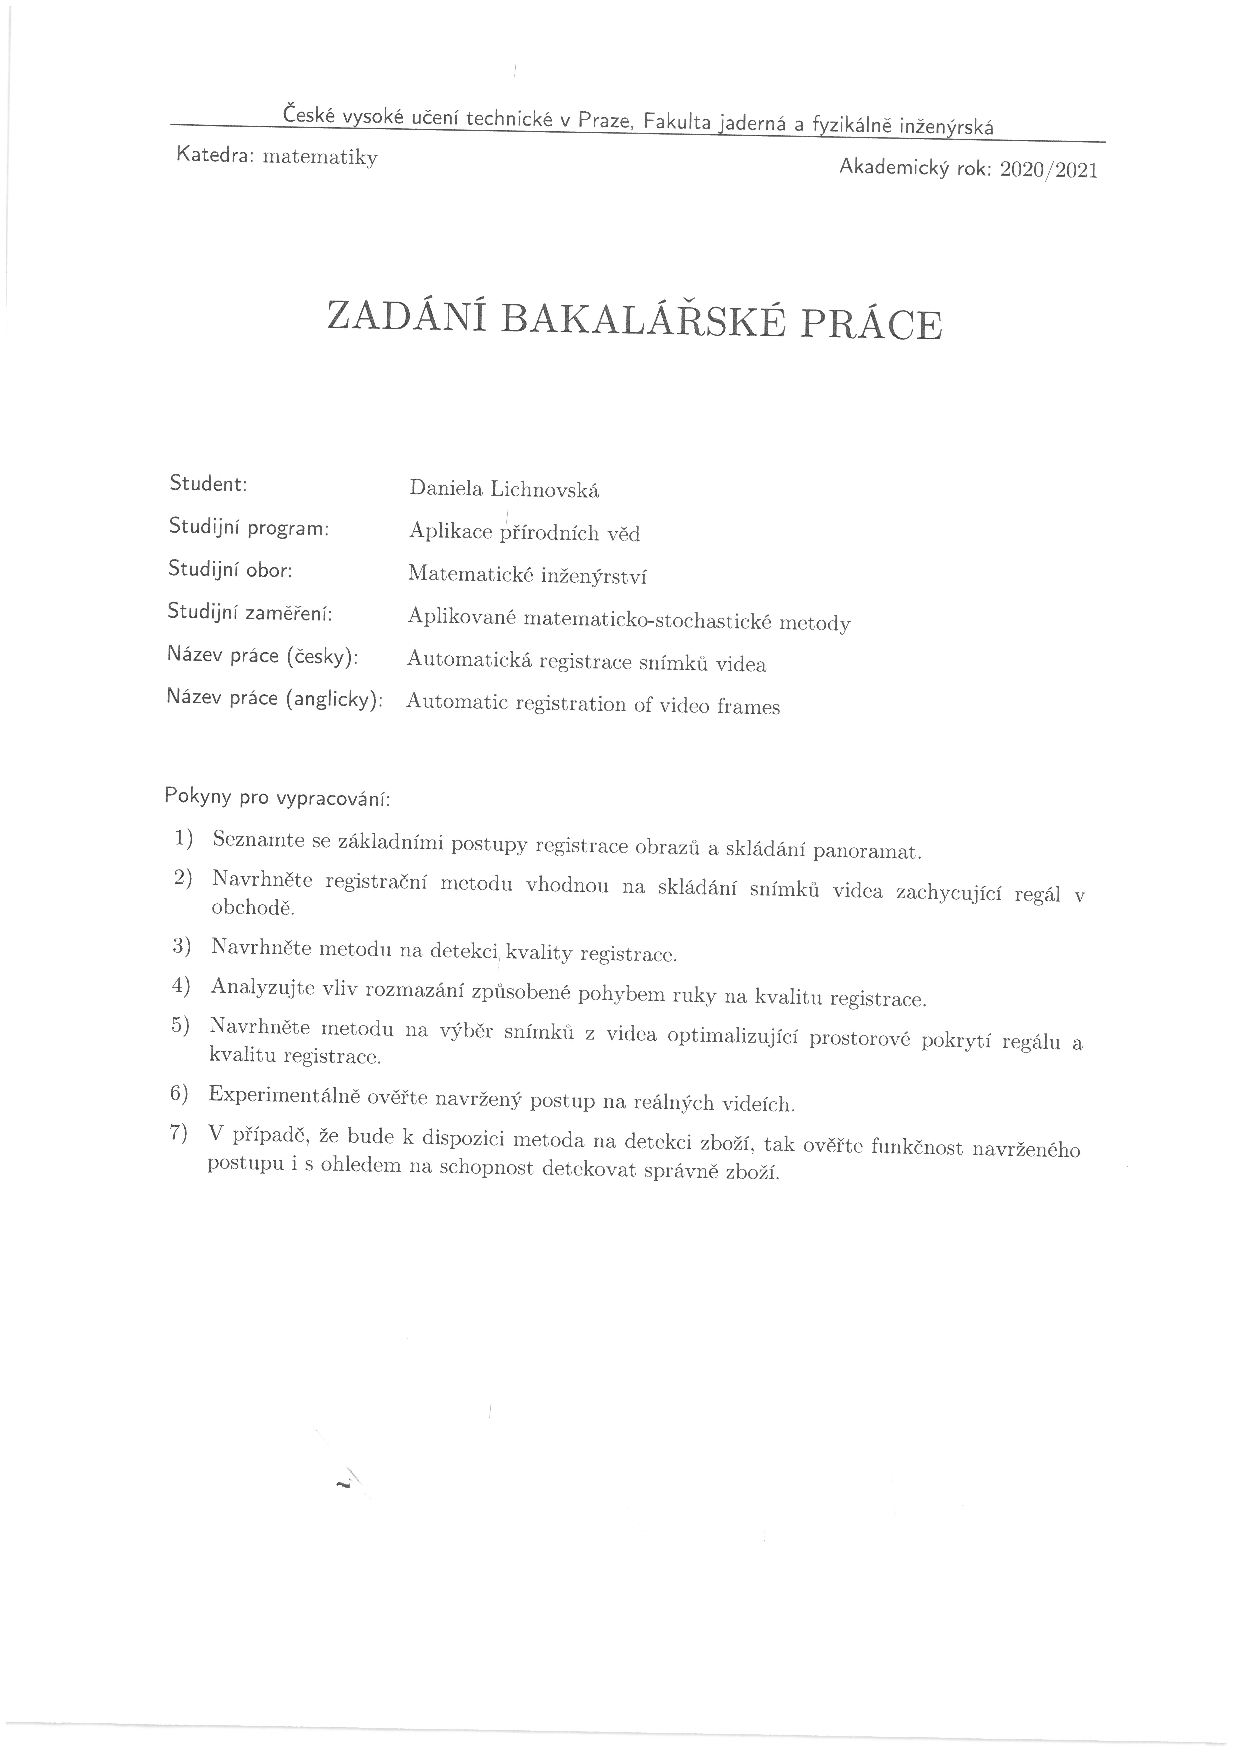
\includepdf[pages=-]{Images/zadani_cele.pdf}

%\vfill{}
%
%\begin{center}
%- Zadání práce -
%\par\end{center}
%
%\vfill{}
%
%~\newpage{}
%
%~
%
%\vfill{}
%
%\begin{center}
%- Zadání práce (zadní strana) -
%\par\end{center}
%
%\vfill{}

%~\newpage{}

\noindent \emph{\Large{}Poděkování:}{\Large\par}

\noindent Chtěl bych zde poděkovat především svému školiteli ...................
za pečlivost, ochotu, vstřícnost a odborné i lidské zázemí při vedení
mé diplomové práce. Dále děkuji svému konzultantovi ................
za ................

\vfill

\noindent \emph{\Large{}Čestné prohlášení:}{\Large\par}

\noindent Prohlašuji, že jsem tuto práci vypracoval samostatně a uvedl
jsem všechnu použitou literaturu.

\bigskip{}

\noindent V Praze dne \documentdate\hfill{}Daniela Lichnovská

\vspace{2cm}

\newpage{}

\begin{onehalfspace}
\noindent \emph{Název práce:}

\noindent \textbf{Název práce}
\end{onehalfspace}

\bigskip{}

\noindent \emph{Autor:} Daniela Lichnovská

\bigskip{}

\noindent \emph{Obor:} Matematické inženýrství\bigskip{}

\noindent \emph{Zaměření:} Aplikované matematicko-stochaistické metody

\bigskip{}

\noindent \emph{Druh práce:} Bakalářská práce

\bigskip{}

\noindent \emph{Vedoucí práce:} doc. Ing. Filip Šroubek, Ph.D. DSc.,
ÚTIA AV ČR Praha, v.v.i.,
Pod Vodárenskou věží 4,
182 00 Praha 8

\bigskip{}

\noindent \emph{Konzultant:} Ing. Lukáš Tryner,
DataSentics, a.s.,
Washingtonova 1599/17,
Praha 1

\bigskip{}

\noindent \emph{Abstrakt:} Abstrakt max. na 10 řádků. Abstrakt max.
na 10 řádků. Abstrakt max. na 10 řádků. Abstrakt max. na 10 řádků.
Abstrakt max. na 10 řádků. Abstrakt max. na 10 řádků. Abstrakt max.
na 10 řádků. Abstrakt max. na 10 řádků. Abstrakt max. na 10 řádků.
Abstrakt max. na 10 řádků. Abstrakt max. na 10 řádků. Abstrakt max.
na 10 řádků. Abstrakt max. na 10 řádků. Abstrakt max. na 10 řádků.
Abstrakt max. na 10 řádků. Abstrakt max. na 10 řádků. Abstrakt max.
na 10 řádků. Abstrakt max. na 10 řádků. Abstrakt max. na 10 řádků.
Abstrakt max. na 10 řádků. Abstrakt max. na 10 řádků. Abstrakt max.
na 10 řádků. Abstrakt max. na 10 řádků. Abstrakt max. na 10 řádků.
Abstrakt max. na 10 řádků. Abstrakt max. na 10 řádků. Abstrakt max.
na 10 řádků. Abstrakt max. na 10 řádků. Abstrakt max. na 10 řádků. 

\bigskip{}

\noindent \emph{Klíčová slova:} klíčová slova (nebo výrazy) seřazená
podle abecedy a oddělená čárkou

\vfill{}
~

\selectlanguage{american}%
\begin{onehalfspace}
\noindent \emph{Title:}

\noindent \textbf{Automatic registration of video frames}
\end{onehalfspace}

\bigskip{}

\noindent \emph{Author:} Daniela Lichnovská

\bigskip{}

\noindent \emph{Abstract:} Max. 10 lines of English abstract text.
Max. 10 lines of English abstract text. Max. 10 lines of English abstract
text. Max. 10 lines of English abstract text. Max. 10 lines of English
abstract text. Max. 10 lines of English abstract text. Max. 10 lines
of English abstract text. Max. 10 lines of English abstract text.
Max. 10 lines of English abstract text. Max. 10 lines of English abstract
text. Max. 10 lines of English abstract text. Max. 10 lines of English
abstract text. Max. 10 lines of English abstract text. Max. 10 lines
of English abstract text. Max. 10 lines of English abstract text.
Max. 10 lines of English abstract text. Max. 10 lines of English abstract
text. Max. 10 lines of English abstract text. Max. 10 lines of English
abstract text. Max. 10 lines of English abstract text. Max. 10 lines
of English abstract text. Max. 10 lines of English abstract text.
Max. 10 lines of English abstract text. Max. 10 lines of English abstract
text. Max. 10 lines of English abstract text.

\bigskip{}

\noindent \emph{Key words:} keywords in alphabetical order separated
by commas

\selectlanguage{czech}%
\newpage{}

\pagestyle{plain}

\tableofcontents{}

\newpage{}

\chapter*{Úvod}

\addcontentsline{toc}{chapter}{Úvod}

Text úvodu....

\chapter{Registrace obrazu}
\pagestyle{headings}
\subsection{co to je}
Registrace obrazu je proces kombinování dvou a více snímků pořízených z odlišných pohledů, času nebo zdrojů do jednoho souřadného sytému \cite{ir_survey}. Je například často používaná při zpracovávání dat ze satelitů,v počítačovém vidění nebo medicíně.

Registraci lze rozdělit do čtyř kroků:
\begin{enumerate}
\item detekce příznaků
\item korespondence příznaků
\item odhad transformace
\item transformace snímku
\end{enumerate}

\section{Detekce příznaků}
\subsection{Metoda SURF}
\subsection{Extrakce příznaků}
\section{Korespondence příznaků}
\section{Estimace modelu transformace}

\subsection{Affiní tr}
\subsection{Projektivní tr}
\section{resamplovaní}
\section{pipeline}

\chapter{Výběr snímků z videa}


\pagestyle{headings}

\section{focus measure}
\section{pocitani chyby v tform}
\section{pipeline}
,
\chapter{experimenty}

\pagestyle{headings}
\section{Opakovatelnost(repeatability)}
Opakovatelnost \cite{repeat}
\section{accuracy}
\section{vliv blur}
\section{vliv komprese}

\chapter{Detekce cenovek}

\pagestyle{headings}



\chapter*{Závěr}

\pagestyle{plain}

\addcontentsline{toc}{chapter}{Záv\v{e}r}

Text závěru....

\printbibliography

\end{document}
